\usetikzlibrary {shapes.geometric}
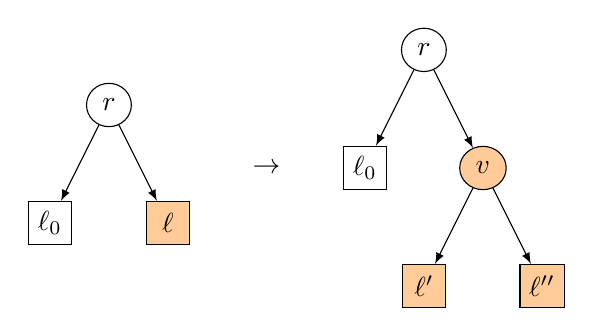
\begin{tikzpicture}[edge from parent/.style={draw,-latex}]
    \tikzset{every node/.style={minimum width=.55cm,minimum height=.55cm}}
    \node [ellipse,draw] {$r$}
        child {node[rectangle,draw] {\texttt{$\ell_0$}}}
        child {node[rectangle,draw,fill=orange!40] {\texttt{$\ell$}}};
    
    \node at (2,-.8) {$\rightarrow$};

    \begin{scope}[xshift=4cm,yshift=.7cm]
        \node [ellipse,draw] {$r$}
        child {node[rectangle,draw] {\texttt{$\ell_0$}}}
        child {node[ellipse,draw,fill=orange!40] {$v$}
            child {node[rectangle,draw,fill=orange!40] {\texttt{$\ell'$}}}
            child {node[rectangle,draw,fill=orange!40] {\texttt{$\ell''$}}}
        };
    \end{scope}

\end{tikzpicture}